\documentclass[handout]{beamer} % [handout] para imprimir eliminando transiciones

%\usefonttheme[onlymath]{serif}
%\usepackage{fontspec}
%\defaultfontfeatures{Mapping=tex-text}
%\setsansfont[Ligatures={Common}]{Futura}
%\setmonofont[Scale=0.8]{Monaco} 

\usepackage{beamerthemesplit}
\usepackage[utf8]{inputenc}
\usepackage[spanish]{babel}
\mode<presentation>
\usetheme{default}
\usecolortheme{dolphin}
\usepackage{alltt}                                    % \begin{alltt}
\usepackage{amssymb}                                  % mathematical symbols
\usepackage{comment}
\usepackage{tabto}                                    % \tabto
\usepackage{tikz}
\usetikzlibrary{automata}
\usetikzlibrary{positioning}
\usetikzlibrary{calc}

\usepackage{verbatim}                                 % comentarios

\title{Lenguajes de Programación}                     %[titulo corto]
\author{Fabián Riquelme Csori}                        %[nombre corto]
\date{2017}                                           %[fecha corta]
\institute{Universidad de Valparaíso}                 %[instituto corto]

\newcommand{\HRule}{\rule{\linewidth}{0.2mm}\\[1ex]}
\newcommand{\blue}[1]{\textcolor{blue}{#1}}
\newcommand{\red}[1]{\textcolor{red}{#1}}
\newcommand{\redb}[1]{{\color{red!70!black}{#1}}}
\newcommand{\green}[1]{{\color{green!70!black}{#1}}}
\newcommand{\gray}[1]{{\color{gray!50!white}{#1}}}
\newcommand{\lQ}{\mbox{``}}
\newcommand{\rQ}{\mbox{''}}
% \alert{texto destacado en rojo}
% \color{green} Color en verde
% \structure{texto en lila}


\begin{document}

%\begin{frame}%[plain]
%  \titlepage
%\end{frame}
%
% [opciones]:
% plain: oculta barra de navegacion, deja + espacio para contenido
% fragile: usar comandos como verbatim
% b,c,t: alineacion vertical
% label=nombre_etiqueta
% allowframebreaks: divide contenido en varios frames si es demasiado largo
% shrink: para escribir mucho texto en una transparencia, reduciendo tamano de fuente

%%%%%%%%%% PORTADA %%%%%%%%%%
\begin{frame}[plain]
  \begin{figure}[h]
    \begin{minipage}{0.3\textwidth}
    
\includegraphics[width=.9\textwidth]{./image/logo-UV.png}
    \end{minipage}
    \begin{minipage}{0.65\textwidth}
     $~$\\[3.6ex]
     \footnotesize{Escuela de Ingeniería Civil Informática}\\
     \footnotesize{Facultad de Ingeniería}
    \end{minipage}
  \end{figure}
  \begin{center}
    \vspace{1ex}
    \HRule
    \Large{Lenguajes de Programación}\\{\small Capítulo III: Análisis semántico}\\[-1ex]
    \HRule\vspace{1ex}
    \large{Fabián Riquelme Csori}\\[.5ex]\footnotesize{fabian.riquelme@uv.cl}\\[6ex] {\tiny 2017-II}\\[6ex]
  \end{center}
\end{frame}

%%%%%%%%%% INDEX %%%%%%%%%%
\begin{frame}
 \frametitle{Index}
 \scriptsize 			% reducir tamano de letra
 \tableofcontents		%[pausesections]
\end{frame}

%%%%%%%%%%% ACTUAL INDEX %%%%%%%%%%
%\AtBeginSection[] %generar indice automaticamente
%{
%\begin{frame}<beamer>%[plain]
% \frametitle{Index}
% \framesubtitle{subtitulo}
% \scriptsize
% \tableofcontents[currentsection, currentsubsection]
%\end{frame}
%}

%==============================
\section{Análisis semántico}

\begin{frame}{Primera fase de compilación}
    \begin{center}
    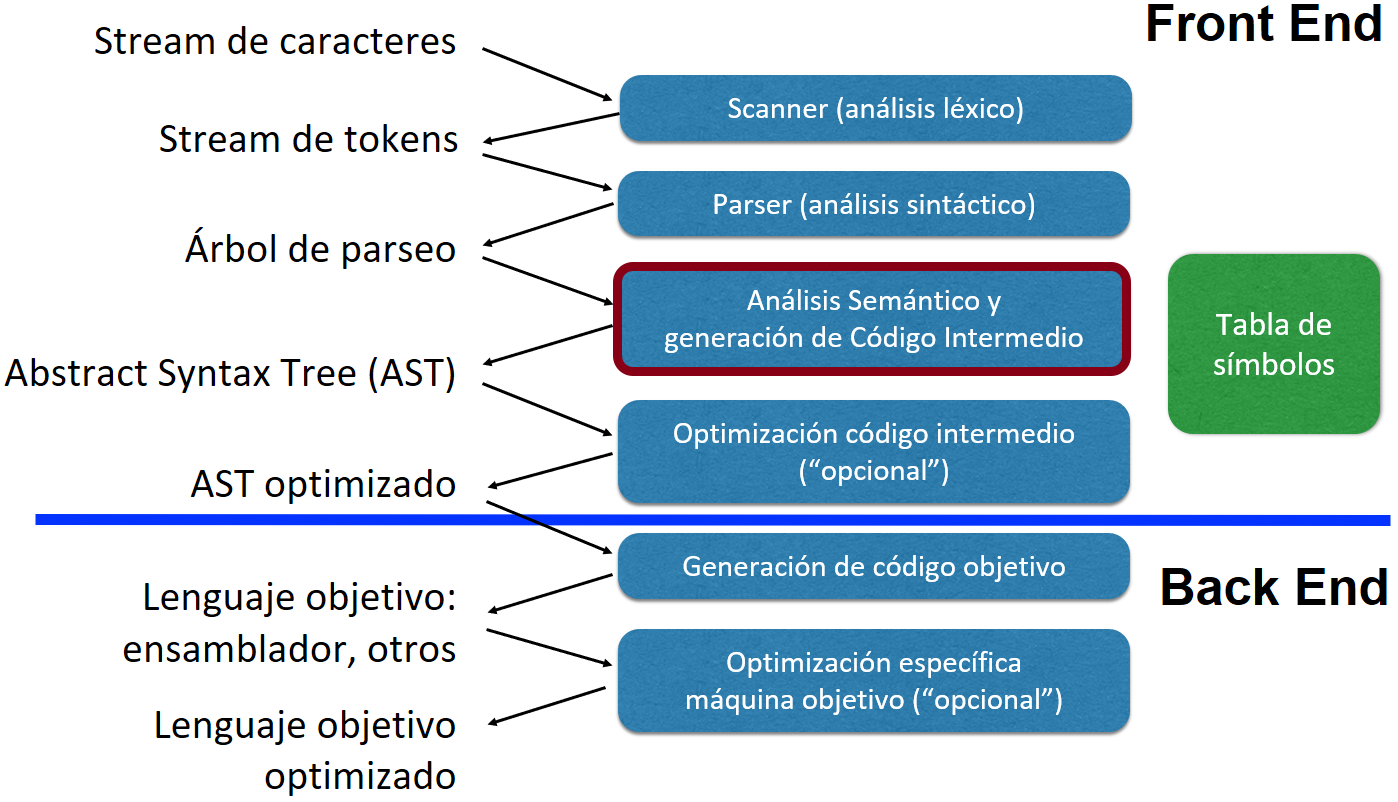
\includegraphics[width=\textwidth]{./image/cap3/compilador-fase3}
    \end{center}
\end{frame}

%------------------------------
\subsection{Representaciones intermedias}

\begin{frame}{Representación Intermedia (IR)}
    \begin{itemize}
        \item<1-> Una \blue{representación intermedia (IR)} o \blue{lenguaje intermedio} es una estructura de datos o código, utilizado internamente por un compilador o máquina virtual, para transitar de un código fuente al código objetivo.
        \item<2-> Como estructura de datos, suele ser un árbol o grafo especial, que representa el flujo de los datos y su orden de precedencia para que luego el compilador genere las instrucciones de CPU.
        \item<3-> Una IR debe ser:
        \begin{itemize}
            \item Certera ({\em accurate}): no perder información.
            \item Independiente del lenguaje objetivo.
        \end{itemize}
        \item<4-> La independencia del lenguaje objetivo permite que una misma IR pueda usarse para compilar códigos diversos y en distintas arquitecturas (Ej: GCC -- GNU Compiler Collection, LLVM -- Low Level Virtual Machine, Java bytecode, etc).
    \end{itemize}
\end{frame}

%------------------------------
\subsection{Árboles de sintaxis abstracta}

\begin{frame}{Árbol de sintaxis abstracta}
    \begin{itemize}
        \item<1-> Una IR muy utilizada por compiladores e intérpretes es la del \blue{árbol de sintaxis abstracta} (\blue{AST}).
        \item<2-> Un AST representa la \blue{sintaxis abstracta} de un código fuente.
        \item<3-> En compiladores, un AST recibe como entrada un \blue{árbol de parseo}, también conocido como \blue{árbol de sintaxis concreta}.
    \end{itemize}
\end{frame}

\begin{frame}{Árbol de sintaxis abstracta}
    \begin{itemize}
        \item<1-> Una IR muy utilizada por compiladores e intérpretes es la del \blue{árbol de sintaxis abstracta} (\blue{AST}).
        \item<2-> Un AST representa la \blue{sintaxis abstracta} de un código fuente.
        \item<3-> En compiladores, un AST recibe como entrada un \blue{árbol de parseo}, también conocido como \blue{árbol de sintaxis concreta}.
    \end{itemize}
\end{frame}

\begin{frame}{AST vs. árbol de parseo}
    \begin{center}
    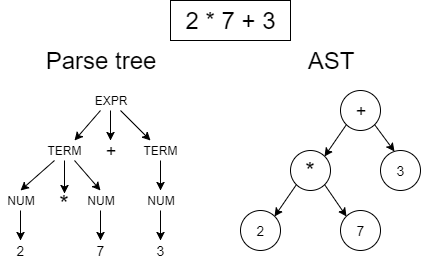
\includegraphics[width=\textwidth]{./image/cap3/AST_parse_tree}
    \end{center}
\end{frame}

\begin{frame}{AST vs. árbol de parseo}
    \begin{itemize}
        \item<1-> Los AST son más compactos y densos que los árboles de parseo
        \begin{itemize}
            \item Ej: probar \blue{7+((2+3))}.
        \end{itemize}
        \item<2-> Los AST tienen en su raíz y nodos internos operadores/ operaciones en lugar de reglas gramaticales/ tokens.
        \item<2-> Los AST se abstraen de los detalles de la sintaxis real\\(Ej: omiten paréntesis).
    \end{itemize}
\end{frame}

\begin{frame}{Ejercicios}
    En los AST, mientras mayor es la precedencia del operador, más inferior es su nivel en el árbol.
    \begin{itemize}
        \item<2-> Construir el AST para \blue{2 * 7 + 3}
        \item<3-> Compararlo con el AST para \blue{2 * (7 + 3)}
        \item<4-> Construir el AST para \blue{1 + 2 + 3 + 4 + 5}
    \end{itemize}
    \uncover<5->{¿Cómo estamos recorriendo el árbol?}
    \medskip
    
    \uncover<6->{¿top-down o bottom-up?}\\
    \uncover<6->{¿por anchura o profundidad (pre-order, in-order, post-order)?}
    \medskip
    
    \uncover<7->{Todas las alternativas son posibles.\\
    El problema de top-down es que puede generar ambigüedades.}
\end{frame}

%------------------------------
\subsection{Propagación de atributos}

\begin{frame}{Propagación de atributos}
    Dada la expresión:\\
    \hspace{3ex} \texttt{int a,b,c;}\\
    \hspace{3ex} \texttt{a/(b+c\string^2)}\\
    El AST es el siguiente:
    \pause
    \begin{center}
    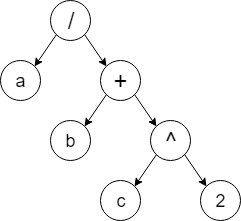
\includegraphics[width=.5\textwidth]{./image/cap3/AST-1}
    \end{center}
\end{frame}

\begin{frame}{Propagación de atributos}
    De la instrucción declarativa, la tabla de símbolos y el analizador sintáctico obtenemos los atributos de los operandos:
    \begin{center}
    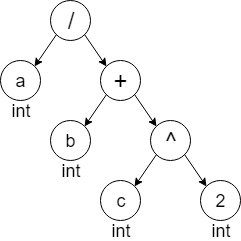
\includegraphics[width=.5\textwidth]{./image/cap3/AST-2}
    \end{center}
\end{frame}

\begin{frame}{Propagación de atributos}
    Propagando los atributos:\\
    
    \begin{center}
    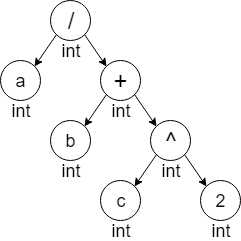
\includegraphics[width=.5\textwidth]{./image/cap3/AST-3}
    \end{center}
\end{frame}

\begin{frame}{Propagación de atributos}
    Si la instrucción fuera \texttt{a/(b+c\string^-2)},\\
    el AST sería el mismo (reemplazando 2 por -2), pero con otra propagación de atributos:
    \begin{center}
    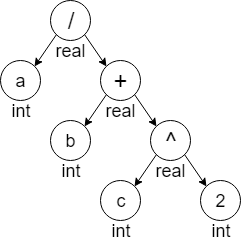
\includegraphics[width=.5\textwidth]{./image/cap3/AST-4}
    \end{center}
\end{frame}

\begin{frame}{Propagación de atributos}
    Si la instrucción fuera \texttt{a/(b+c\string^d)}:\\
    \begin{center}
    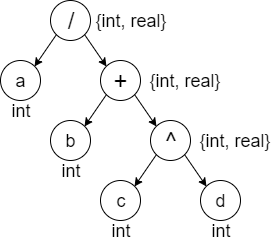
\includegraphics[width=.5\textwidth]{./image/cap3/AST-5}
    \end{center}
    El analizador semántico puede escoger el tipo de datos más flexible (real) o definir uno nuevo.
\end{frame}

\begin{frame}{Ejemplo}
    \begin{center}
    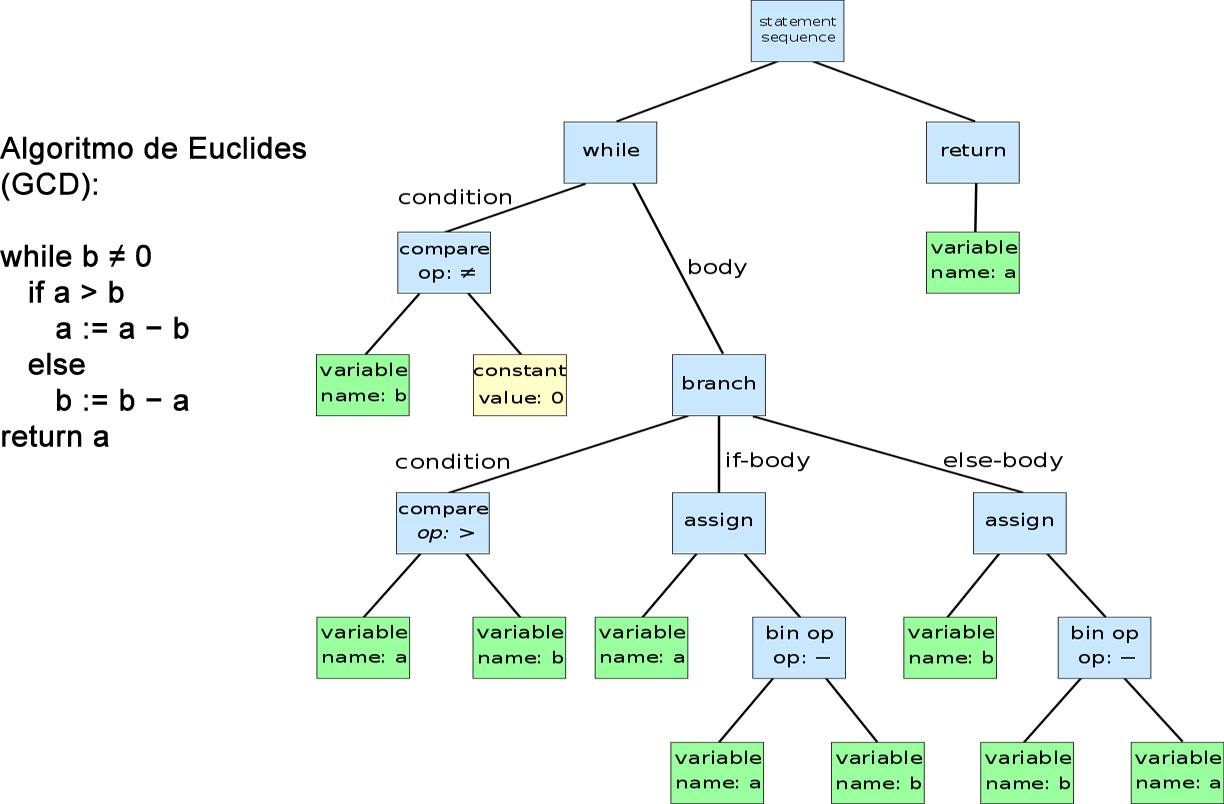
\includegraphics[width=\textwidth]{./image/cap3/AST-euclidean}
    \end{center}
\end{frame}

%------------------------------

\begin{frame}
 \begin{block}{Bibliografía}
  \begin{itemize}
    \item Pratt, Terrence W. (1998). \textit{Lenguajes de programación: diseño e implementación}, Pearson Education.
    \item Sethi, Ravi (1992). \textit{Lenguajes de programación: conceptos y constructores}, Addison-Wesley Iberoamericana.
    \item Scott, Michael (2009). \textit{Programming Language Pragmatics}, Morgan Kaufman, 3ra ed.
  \end{itemize}
 \end{block}
 \begin{block}{Recursos}
  \begin{itemize}
    \item Wikipedia y Wikimedia Commons.
    \item Imágenes con licencia libre.
  \end{itemize}
 \end{block}
\end{frame}

\end{document}
